\subsection{Use case view}
\subsubsection{Gestion des utilisateurs}
{\noindent L'utilisateur, désireux de jouer, devra d'abord s'enregistrer dans le \index{système}système. Pour ce faire, il lui faudra introduire un identifiant et un mot de passe. Certaines contraintes pour assurer la sécurité des comptes de jeu. L'identifiant devra être unique dans le \index{système}système. Une fois l'étape complétée, le compte de jeu sera créé et stocké dans le \index{système}système.}
\subsubsection{Connexion}
{\noindent Pour se connecter, l'utilisateur devra utiliser son identifiant et son mot de passe enregistrés dans le \index{système}système. Il fera alors une demande au \index{système}système qui va vérifier si le compte est bien introduit. Si la connexion échoue, un message signalera l'endroit de l'erreur. Si la connexion réussi, l'utilisateur aura accès au menu principal et pourra commencer à jouer.
}

\subsubsection{Créer un deck}
{\noindent L'utilisateur a la possibilité de créer ses propres \index{deck}decks. Ces \index{deck}decks seront créés via la \index{collection}collection de l'utilisateur et sera associé à son \index{account}account. Il pourra enregistrer un certain nombre de \index{deck}deck et en choisir un actif. Le \index{deck}deck actif sera utilisé lors du prochain \index{duel}duel de l'utilisateur.
}

\subsubsection{Matchmaking}
{\noindent Le matchmaking va s'occuper de créer la relation entre les deux adversaires. La recherche d'aversaire est totalement aléatoire, elle n'est pas affecté par les stats des \index{account}accounts. Un player ayant une série de 500 victoires pourrait tomber sur un nouveau joueur découvrant le jeu. Le monde de Wizard Poker n'est pas toujours juste.
}

\newpage
\subsubsection{Jouer un tour}
{\noindent A chaque tour de jeu, la main est donné à un des Players. Le Player dont c'est le tour pourra utiliser les cartes qu'il a en main ainsi que ces Minions en jeu. L'autre joueur devra attendre mais pourra tout de même entre-temps discuter avec ces amis. Nous proposons un diagramme use case pour illustrer cette situation.\\
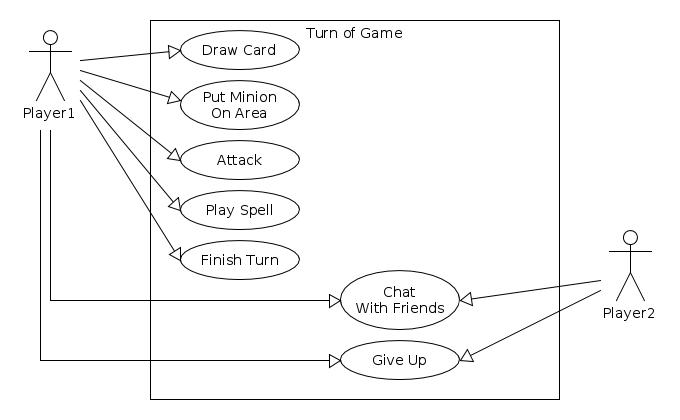
\includegraphics[width=0.8\textwidth]{Images/UseCaseGame.jpg}
}
\subsubsection{Déclarer forfait}
{\noindent Tout le monde s'est déjà rendu dans une situation où la victoire n'est plus du tout envisageable. Afin de gagner du temps, l'utilisateur aura la possibilité de déclarer forfait\index{forfait}. Ceci mettra donc un terme à la partie en cours.}

\section{Exigences non fonctionnelles}
\section{Design et fonctionnement du système}
\subsection{Diagramme de Classes}
{
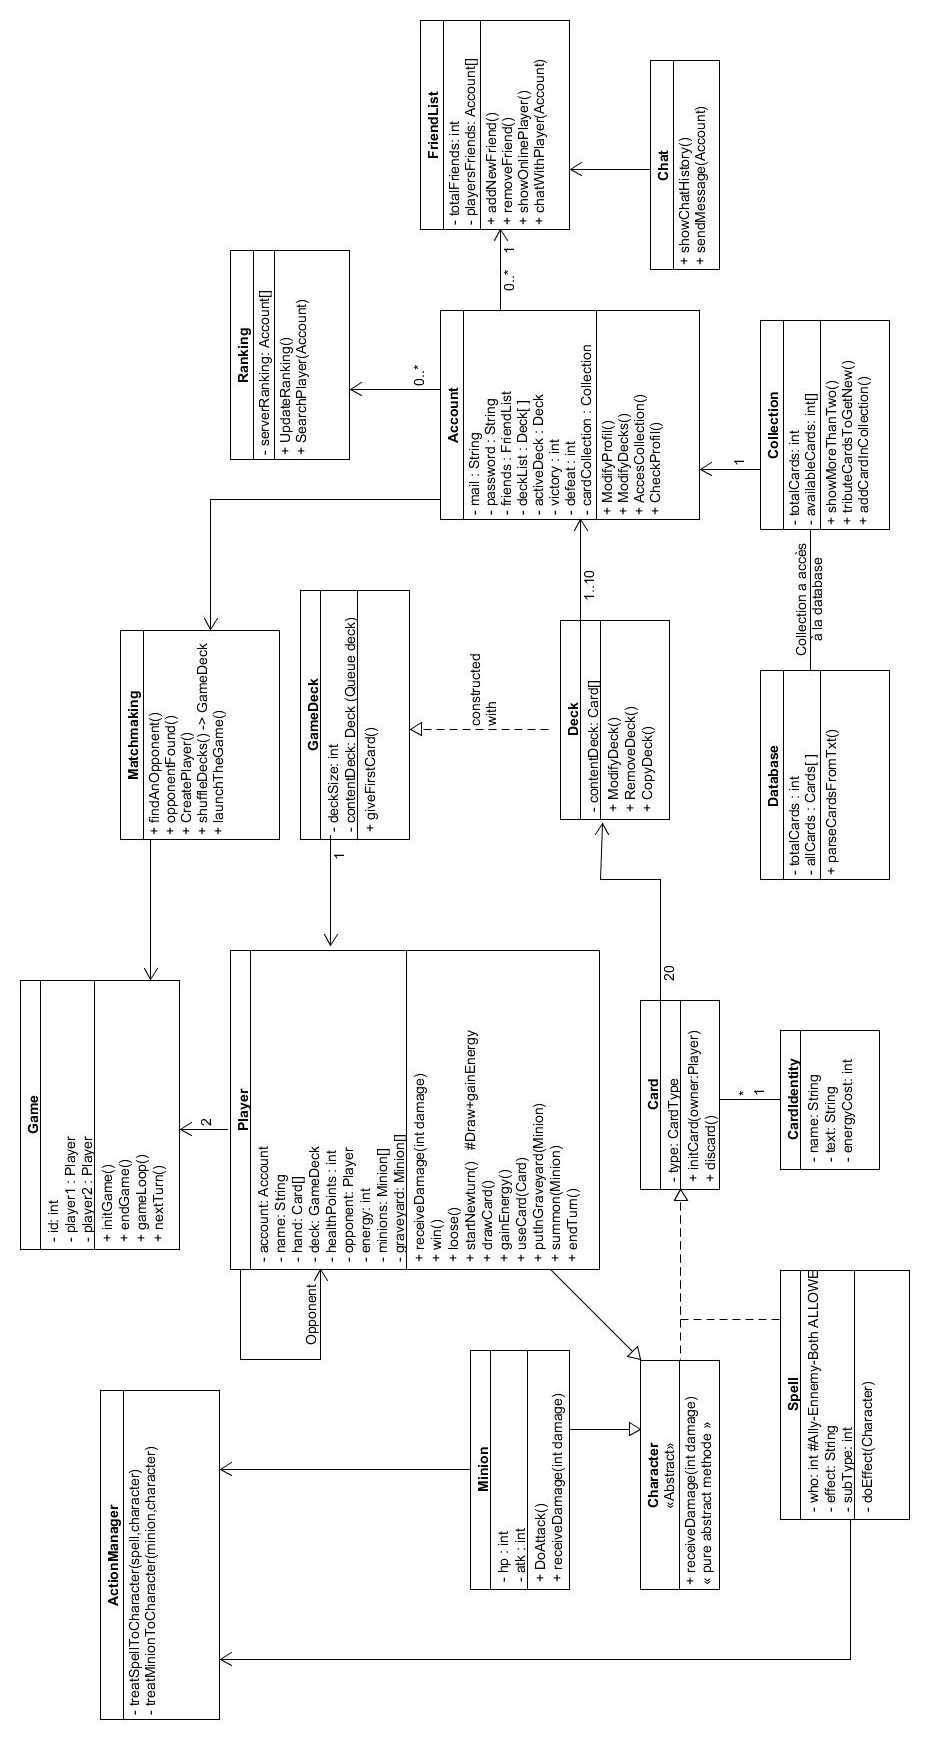
\includegraphics[width=1.1\textwidth,height=1.3\textwidth]{Images/ClassDiagramV.jpg}
}
\subsubsection{Analyse globale}
{\noindent Dans ce diagramme se trouve un aperçu globale de l'application. Le projet devant être codé principalement en orienté-objet, nous avons divisé le problème en un maximum de classe. Les méthodes et attributs ont des signatures adaptés pour permettre au client de comprendre la tache effectué par chaque classe. Le diagramme est sensé être claire, mais il y a certains points qui méritent plus de précisions.}
\subsubsection{ActionManager}
{\noindent C'est dans cette classe que va se dérouler les actions. Une action peut être de 2 types. La première est provoqué par le {minion} de l'un des player qui va attaquer un character\index{character} adverse. La deuxième sera provoqué lors de l'utilisation d'un {spell} qui va cibler un character\index{character} adverse.\\
Ces deux actions ont un effet différents. Dans le premier, il y a le \index{système}système de {contre-attaque} qui implique une modification du character\index{character} qui se fait attaqué mais le {minion} qui attaque également, si le character\index{character} en question a une attaque plus grande que 0. Tandis que dans le cas d'un {spell}, c'est seulement le character\index{character} visé qui sera modifié, le {spell} quant à lui sera défaussé de la main.}
\subsubsection{Database}
{\noindent Pour conserver les cartes, nous avons décider d'enregistrer toutes les cartes du jeu dans un fichier texte avec une syntaxe précise. Celle-ci sera donc chargé lors de l'ouverture du jeu. Lorsqu'un joueur veut accéder à sa \index{collection}collection, celle-ci sera trouvé depuis la Database. Nous voyons la Database comme la liste de toutes les cartes disponibles, de la sorte chaque joueur aura sa propre vision sur la disponibilité d'une carte. De la sorte, il ne faudra pas copier chaque carte dans la \index{collection}collection de chaque joueur, mais seulement déterminer pour chaque joueur, si une carte est disponible ou non.}